\documentclass{standalone}
\usepackage{tikz}
\usetikzlibrary{patterns, positioning}


\begin{document}
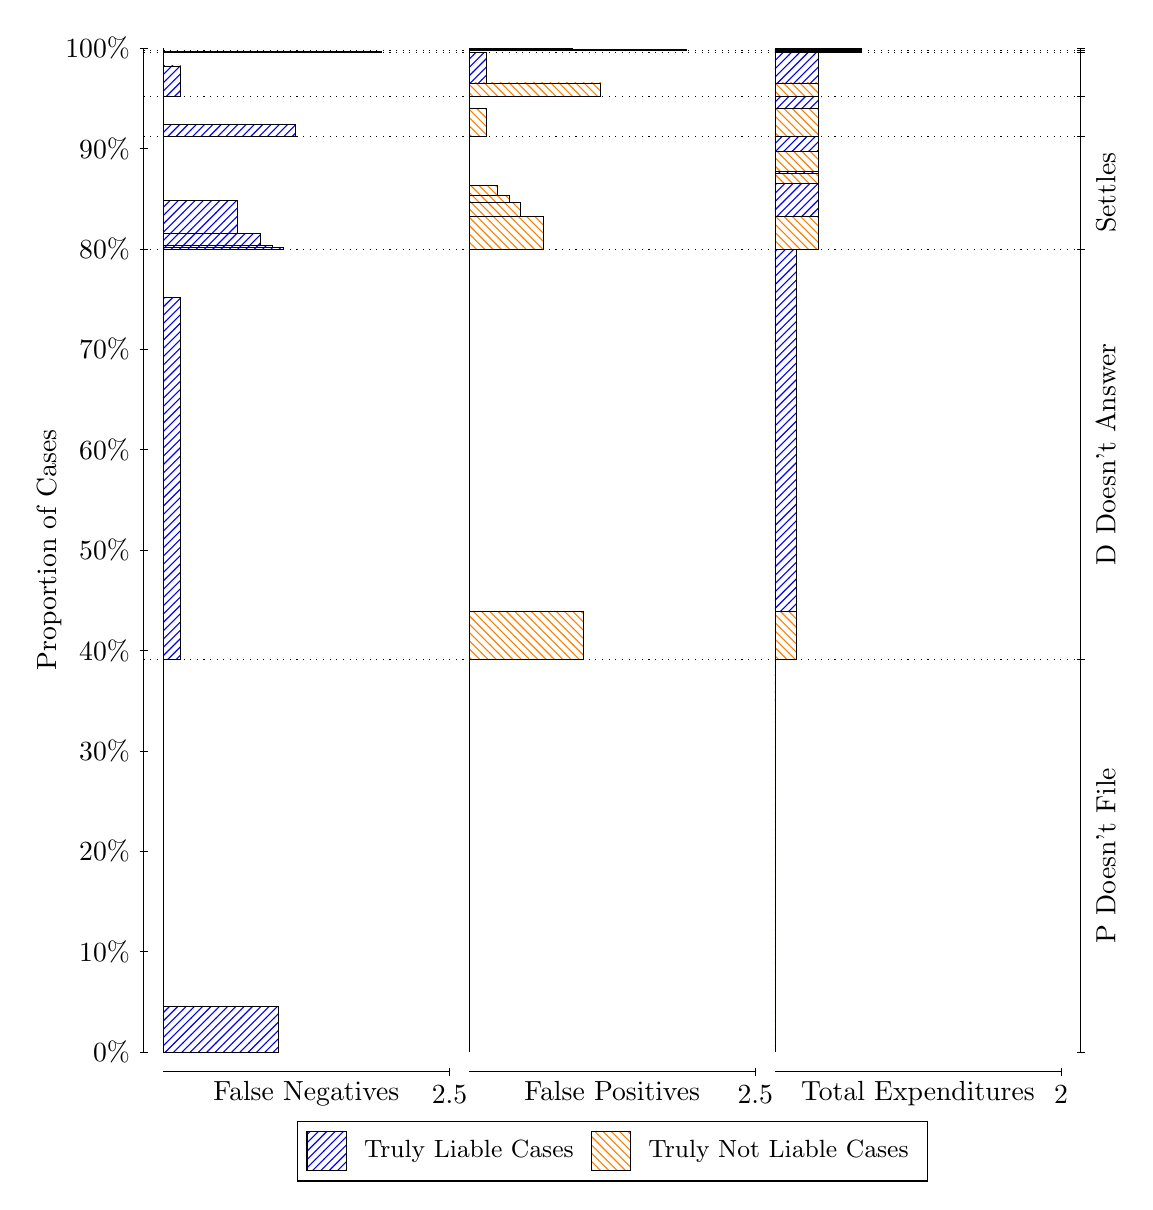
\begin{tikzpicture}
\draw[black, very thin] (1.5,1.75) -- (1.5,14.5);
\node[rotate=90, text=black, anchor=center] at (0.3, 8.125) {Proportion of Cases};
\draw[black, very thin] (1.45,1.75) -- (1.55,1.75);
\node[text=black, anchor=east] at (1.45, 1.75) {0\%};
\draw[black, very thin] (1.45,3.025) -- (1.55,3.025);
\node[text=black, anchor=east] at (1.45, 3.025) {10\%};
\draw[black, very thin] (1.45,4.3) -- (1.55,4.3);
\node[text=black, anchor=east] at (1.45, 4.3) {20\%};
\draw[black, very thin] (1.45,5.575) -- (1.55,5.575);
\node[text=black, anchor=east] at (1.45, 5.575) {30\%};
\draw[black, very thin] (1.45,6.85) -- (1.55,6.85);
\node[text=black, anchor=east] at (1.45, 6.85) {40\%};
\draw[black, very thin] (1.45,8.125) -- (1.55,8.125);
\node[text=black, anchor=east] at (1.45, 8.125) {50\%};
\draw[black, very thin] (1.45,9.4) -- (1.55,9.4);
\node[text=black, anchor=east] at (1.45, 9.4) {60\%};
\draw[black, very thin] (1.45,10.675) -- (1.55,10.675);
\node[text=black, anchor=east] at (1.45, 10.675) {70\%};
\draw[black, very thin] (1.45,11.95) -- (1.55,11.95);
\node[text=black, anchor=east] at (1.45, 11.95) {80\%};
\draw[black, very thin] (1.45,13.225) -- (1.55,13.225);
\node[text=black, anchor=east] at (1.45, 13.225) {90\%};
\draw[black, very thin] (1.45,14.5) -- (1.55,14.5);
\node[text=black, anchor=east] at (1.45, 14.5) {100\%};

\draw[black, very thin] (13.4,1.75) -- (13.4,14.5);
\draw[black, very thin] (13.35,1.75) -- (13.45,1.75);
\node[anchor=west] at (13.35, 1.75) {};
\draw[black, very thin] (13.35,6.7367) -- (13.45,6.7367);
\node[anchor=west] at (13.35, 6.7367) {};
\draw[black, very thin] (13.35,11.944) -- (13.45,11.944);
\node[anchor=west] at (13.35, 11.944) {};
\draw[black, very thin] (13.35,13.38) -- (13.45,13.38);
\node[anchor=west] at (13.35, 13.38) {};
\draw[black, very thin] (13.35,13.883) -- (13.45,13.883);
\node[anchor=west] at (13.35, 13.883) {};
\draw[black, very thin] (13.35,14.447) -- (13.45,14.447);
\node[anchor=west] at (13.35, 14.447) {};
\draw[black, very thin] (13.35,14.474) -- (13.45,14.474);
\node[anchor=west] at (13.35, 14.474) {};
\draw[black, very thin] (13.35,14.5) -- (13.45,14.5);
\node[anchor=west] at (13.35, 14.5) {};

\draw[black, very thin, pattern color=blue, pattern=north east lines] (1.75,1.75) rectangle (3.2033,2.3318);
\draw[black, very thin, pattern color=orange, pattern=north west lines] (1.75,2.3318) rectangle (1.75,6.7367);
\draw[black, very thin, pattern color=blue, pattern=north east lines] (1.75,6.7367) rectangle (1.968,11.338);
\draw[black, very thin, pattern color=orange, pattern=north west lines] (1.75,11.338) rectangle (1.75,11.944);
\draw[black, very thin, pattern color=blue, pattern=north east lines] (1.75,11.944) rectangle (3.276,11.964);
\draw[black, very thin, pattern color=blue, pattern=north east lines] (1.75,11.964) rectangle (3.1307,11.992);
\draw[black, very thin, pattern color=blue, pattern=north east lines] (1.75,11.992) rectangle (2.9853,12.149);
\draw[black, very thin, pattern color=blue, pattern=north east lines] (1.75,12.149) rectangle (2.6947,12.567);
\draw[black, very thin, pattern color=orange, pattern=north west lines] (1.75,12.567) rectangle (1.75,13.38);
\draw[black, very thin, pattern color=blue, pattern=north east lines] (1.75,13.38) rectangle (3.4213,13.533);
\draw[black, very thin, pattern color=orange, pattern=north west lines] (1.75,13.533) rectangle (1.75,13.883);
\draw[black, very thin, pattern color=blue, pattern=north east lines] (1.75,13.883) rectangle (1.968,14.273);
\draw[black, very thin, pattern color=orange, pattern=north west lines] (1.75,14.273) rectangle (1.75,14.447);
\draw[black, very thin, pattern color=blue, pattern=north east lines] (1.75,14.447) rectangle (4.5113,14.46);
\draw[black, very thin, pattern color=orange, pattern=north west lines] (1.75,14.46) rectangle (1.75,14.474);
\draw[black, very thin, pattern color=orange, pattern=north west lines] (1.75,14.474) rectangle (1.75,14.486);
\draw[black, very thin, pattern color=blue, pattern=north east lines] (1.75,14.486) rectangle (1.75,14.5);
\draw[black, very thin, pattern color=orange, pattern=north west lines] (5.6333,1.75) rectangle (5.6333,6.155);
\draw[black, very thin, pattern color=blue, pattern=north east lines] (5.6333,6.155) rectangle (5.6333,6.7367);
\draw[black, very thin, pattern color=orange, pattern=north west lines] (5.6333,6.7367) rectangle (7.0867,7.343);
\draw[black, very thin, pattern color=blue, pattern=north east lines] (5.6333,7.343) rectangle (5.6333,11.944);
\draw[black, very thin, pattern color=orange, pattern=north west lines] (5.6333,11.944) rectangle (6.578,12.362);
\draw[black, very thin, pattern color=orange, pattern=north west lines] (5.6333,12.362) rectangle (6.2873,12.538);
\draw[black, very thin, pattern color=orange, pattern=north west lines] (5.6333,12.538) rectangle (6.142,12.625);
\draw[black, very thin, pattern color=orange, pattern=north west lines] (5.6333,12.625) rectangle (5.9967,12.757);
\draw[black, very thin, pattern color=blue, pattern=north east lines] (5.6333,12.757) rectangle (5.6333,13.38);
\draw[black, very thin, pattern color=orange, pattern=north west lines] (5.6333,13.38) rectangle (5.8513,13.73);
\draw[black, very thin, pattern color=blue, pattern=north east lines] (5.6333,13.73) rectangle (5.6333,13.883);
\draw[black, very thin, pattern color=orange, pattern=north west lines] (5.6333,13.883) rectangle (7.3047,14.057);
\draw[black, very thin, pattern color=blue, pattern=north east lines] (5.6333,14.057) rectangle (5.8513,14.447);
\draw[black, very thin, pattern color=orange, pattern=north west lines] (5.6333,14.447) rectangle (5.6333,14.461);
\draw[black, very thin, pattern color=blue, pattern=north east lines] (5.6333,14.461) rectangle (5.6333,14.474);
\draw[black, very thin, pattern color=orange, pattern=north west lines] (5.6333,14.474) rectangle (8.3947,14.486);
\draw[black, very thin, pattern color=blue, pattern=north east lines] (5.6333,14.486) rectangle (6.9413,14.5);
\draw[black, very thin, pattern color=orange, pattern=north west lines] (9.5167,1.75) rectangle (9.5167,6.155);
\draw[black, very thin, pattern color=blue, pattern=north east lines] (9.5167,6.155) rectangle (9.5167,6.7367);
\draw[black, very thin, pattern color=orange, pattern=north west lines] (9.5167,6.7367) rectangle (9.7892,7.343);
\draw[black, very thin, pattern color=blue, pattern=north east lines] (9.5167,7.343) rectangle (9.7892,11.944);
\draw[black, very thin, pattern color=orange, pattern=north west lines] (9.5167,11.944) rectangle (10.062,12.362);
\draw[black, very thin, pattern color=blue, pattern=north east lines] (9.5167,12.362) rectangle (10.062,12.78);
\draw[black, very thin, pattern color=orange, pattern=north west lines] (9.5167,12.78) rectangle (10.062,12.912);
\draw[black, very thin, pattern color=blue, pattern=north east lines] (9.5167,12.912) rectangle (10.062,12.932);
\draw[black, very thin, pattern color=orange, pattern=north west lines] (9.5167,12.932) rectangle (10.062,13.195);
\draw[black, very thin, pattern color=blue, pattern=north east lines] (9.5167,13.195) rectangle (10.062,13.38);
\draw[black, very thin, pattern color=orange, pattern=north west lines] (9.5167,13.38) rectangle (10.062,13.73);
\draw[black, very thin, pattern color=blue, pattern=north east lines] (9.5167,13.73) rectangle (10.062,13.883);
\draw[black, very thin, pattern color=orange, pattern=north west lines] (9.5167,13.883) rectangle (10.062,14.057);
\draw[black, very thin, pattern color=blue, pattern=north east lines] (9.5167,14.057) rectangle (10.062,14.447);
\draw[black, very thin, pattern color=orange, pattern=north west lines] (9.5167,14.447) rectangle (10.607,14.461);
\draw[black, very thin, pattern color=blue, pattern=north east lines] (9.5167,14.461) rectangle (10.607,14.474);
\draw[black, very thin, pattern color=orange, pattern=north west lines] (9.5167,14.474) rectangle (10.607,14.486);
\draw[black, very thin, pattern color=blue, pattern=north east lines] (9.5167,14.486) rectangle (10.607,14.5);
\draw[black, dotted] (1.5,6.7367) -- (13.4,6.7367);
\draw[black, dotted] (1.5,11.944) -- (13.4,11.944);
\draw[black, dotted] (1.5,13.38) -- (13.4,13.38);
\draw[black, dotted] (1.5,13.883) -- (13.4,13.883);
\draw[black, dotted] (1.5,14.447) -- (13.4,14.447);
\draw[black, dotted] (1.5,14.474) -- (13.4,14.474);
\draw[black, very thin] (1.75,1.5) -- (5.3833,1.5);
\node[text=black, anchor=north] at (3.5667, 1.5) {False Negatives};
\draw[black, very thin] (5.3833,1.45) -- (5.3833,1.55);
\node[text=black, anchor=north] at (5.3833, 1.45) {2.5};

\draw[black, very thin] (5.6333,1.5) -- (9.2667,1.5);
\node[text=black, anchor=north] at (7.45, 1.5) {False Positives};
\draw[black, very thin] (9.2667,1.45) -- (9.2667,1.55);
\node[text=black, anchor=north] at (9.2667, 1.45) {2.5};

\draw[black, very thin] (9.5167,1.5) -- (13.15,1.5);
\node[text=black, anchor=north] at (11.333, 1.5) {Total Expenditures};
\draw[black, very thin] (13.15,1.45) -- (13.15,1.55);
\node[text=black, anchor=north] at (13.15, 1.45) {2};

\node[text=black, centered, rotate=90] at (13.72, 4.2434) {P Doesn't File};
\node[text=black, centered, rotate=90] at (13.72, 9.3403) {D Doesn't Answer};
\node[text=black, centered, rotate=90] at (13.72, 12.662) {Settles};





\draw (7.449999999999999,1.5) node[draw=none] (baseCoordinate) {};
\begin{scope}[align=center]
        \matrix[scale=0.5, draw=black, below=0.5cm of baseCoordinate, nodes={draw}, column sep=0.1cm]{
            \node[rectangle, draw, minimum width=0.5cm, minimum height=0.5cm, pattern color=blue, pattern=north east lines] {}; &
            \node[draw=none, font=\small, text=black] (B) {Truly Liable Cases}; &
            \node[rectangle, draw, minimum width=0.5cm, minimum height=0.5cm, pattern color=orange, pattern=north west lines] {}; &
            \node[draw=none, font=\small, text=black] (B) {Truly Not Liable Cases}; \\
            };
\end{scope}

\end{tikzpicture}
\end{document}